
        \documentclass[addpoints,spanish, 12pt,a4paper]{exam}
        %\documentclass[answers, spanish, 12pt,a4paper]{exam}
        
        \pointpoints{punto}{puntos}
        \hpword{Puntos:}
        \vpword{Puntos:}
        \htword{Total}
        \vtword{Total}
        \hsword{Resultado:}
        \hqword{Ejercicio:}
        \vqword{Ejercicio:}

        \usepackage[utf8]{inputenc}
        \usepackage[spanish]{babel}
        \usepackage{eurosym}
        %\usepackage[spanish,es-lcroman, es-tabla, es-noshorthands]{babel}


        \usepackage[margin=1in]{geometry}
        \usepackage{amsmath,amssymb}
        \usepackage{multicol, xparse}

        \usepackage{yhmath}

        \usepackage{verbatim}
        %\usepackage{pstricks}


        \usepackage{graphicx}
        \graphicspath{{../img/}}




        \let\multicolmulticols\multicols
        \let\endmulticolmulticols\endmulticols
        \RenewDocumentEnvironment{multicols}{mO{}}
         {%
          \ifnum#1=1
            #2%
          \else % More than 1 column
            \multicolmulticols{#1}[#2]
          \fi
         }
         {%
          \ifnum#1=1
          \else % More than 1 column
            \endmulticolmulticols
          \fi
         }
        \renewcommand{\solutiontitle}{\noindent\textbf{Sol:}\enspace}

        \newcommand{\samedir}{\mathbin{\!/\mkern-5mu/\!}}

        \newcommand{\class}{1º Bachillerato}
        \newcommand{\examdate}{\today}

        %\newcommand{\tipo}{A}


        \newcommand{\timelimit}{50 minutos}

        \renewcommand{\solutiontitle}{\noindent\textbf{Solución:}\enspace}


        \pagestyle{head}
        \firstpageheader{
\includegraphics[width=0.2\columnwidth]{header_left}}{\textbf{Departamento de Matemáticas\linebreak \class}\linebreak \examnum}{
\includegraphics[width=0.1\columnwidth]{header_right}}
        \runningheader{\class}{\examnum}{Página \thepage\ of \numpages}
        \runningheadrule
        
        \pointsinrightmargin % Para poner las puntuaciones a la derecha. Se puede cambiar. Si se comenta, sale a la izquierda.
        \extrawidth{-2.4cm} %Un poquito más de margen por si ponemos textos largos.
        \marginpointname{ \emph{\points}}

        %\printanswers
            \newcommand{\tipo}{A}\newcommand{\examnum}{Auto evaluación 2 - 1ª evaluación}
        \begin{document}
        \noindent
        \begin{tabular*}{\textwidth}{l @{\extracolsep{\fill}} r @{\extracolsep{6pt}} }
        \textbf{Nombre:} \makebox[3.5in]{\hrulefill} & \textbf{Fecha:}\makebox[1in]{\hrulefill} \\
         & \\
        \textbf{Tiempo: \timelimit} & Tipo: \tipo 
        \end{tabular*}
        \rule[2ex]{\textwidth}{2pt}
        Esta prueba tiene \numquestions\ ejercicios. La puntuación máxima es de \numpoints. 
        La nota final de la prueba será la parte proporcional de la puntuación obtenida sobre la puntuación máxima. 

        \begin{center}


        \addpoints
             %\gradetable[h][questions]
            \pointtable[h][questions]
        \end{center}

        \noindent
        \rule[2ex]{\textwidth}{2pt}

        \begin{questions}
        \question Efectúa simplificando el resultado si es posible:
        \begin{multicols}{1} 
        \begin{parts} \part[1]  $ \frac{1}{{\frac{{x + 1}}{{x - 1}} - \frac{{x - 1}}{{x + 1}}}} $  \begin{solution}  $ \frac{x^{2} - 1}{4 x} $  \end{solution} \part[1]  $ ( {{x^3} + x} )\cdot( {1 - \frac{{2x}}{{2x + \frac{2}{x}}}}) $  \begin{solution}  $ x $  \end{solution}
        \end{parts}
        \end{multicols}
        \question Resuelve mediante expresiones algebraicas y Gauss:
        \begin{multicols}{1} 
        \begin{parts} \part[1] Un librero vendió 84 libros, unos a 45 euros y otros a 36 y obtuvo de la venta 3.105 euros. ¿Cuántos vendió de
cada clase?  \begin{solution}  $ \left\{\begin{matrix}3105=45x+36y\\ 84=x+y\\ \end{matrix}\right.  \rightarrow  \\\left[\begin{matrix}36 & 45 & 3105\\0 & - \frac{1}{4} & - \frac{9}{4}\end{matrix}\right] \rightarrow  \left \{ x : 9, \quad y : 75\right \} $  \end{solution} \part[1] En un corral hay conejos y gallinas, en total 50 cabezas y 140 patas. 
    ¿Cuántos animales hay de cada clase?  \begin{solution}  $ \left\{\begin{matrix}50=x+y\\ 140=4x+2y\\ \end{matrix}\right.  \rightarrow  \\\left[\begin{matrix}1 & 1 & 50\\0 & 2 & 40\end{matrix}\right] \rightarrow  \left \{ x : 20, \quad y : 30\right \} $  \end{solution}
        \end{parts}
        \end{multicols}
        \question Discute y resuelve los sistemas:
        \begin{multicols}{1} 
        \begin{parts} \part[1]  $ \left\{\begin{matrix}x+y+z=1\\ x + 2y - z = 2\\ 2x +3y = 4\\ \end{matrix}\right. $  \begin{solution}  $ \left[\begin{matrix}1 & 1 & 1 & 1\\0 & -1 & -3 & 0\\0 & 0 & 0 & 1\end{matrix}\right] \rightarrow  \\ \left [ \right ] $  \end{solution} \part[1]  $ \left\{\begin{matrix}x - y + z = 5\\ \frac{{x - 1}}{2} + \frac{y}{3} = 1\\ \frac{{2x + y}}{2} - \frac{{3z + y}}{3} = 4\\ \end{matrix}\right. $  \begin{solution}  $ \left[\begin{matrix}-1 & 1 & 1 & 5\\0 & \frac{5}{6} & \frac{1}{3} & \frac{19}{6}\\0 & 0 & - \frac{13}{10} & \frac{2}{5}\end{matrix}\right] \rightarrow  \\ \left \{ x : \frac{51}{13}, \quad y : - \frac{18}{13}, \quad z : - \frac{4}{13}\right \} $  \end{solution}
        \end{parts}
        \end{multicols}
        \question Resuelve los siguientes sistemas de inecuaciones:
        \begin{multicols}{1} 
        \begin{parts} \part[1]  $ \left\{\begin{matrix}\frac{{x - 1}}{2} - \frac{{x + 3}}{3} \leq x\\ \frac{{4x - 2}}{4} - \frac{{x - 1}}{3} \geq x\end{matrix}\right. $  \begin{solution}  $ \left[- \frac{9}{5}, - \frac{1}{2}\right] $  \end{solution} \part[1]  $ \left\{\begin{matrix}\frac{{3( {2 - x} )}}{2} - x < \frac{{16}}{3} - \frac{{x + 1}}{5} \\\frac{{x + 4}}{3} - \frac{{x - 5}}{6} > 3 - \frac{{2x - 3}}{{18}}\end{matrix}\right. $  \begin{solution}  $ \left(\frac{18}{5}, \infty\right) $  \end{solution}
        \end{parts}
        \end{multicols}
        \question Resuelve los siguientes sistemas de inecuaciones:
        \begin{multicols}{1} 
        \begin{parts} \part[1]  $ \left\{\begin{matrix}- 2 \leq x\\x \leq 2\\y \geq 4\\x + y - 1 \leq 0\\\end{matrix}\right. $  \begin{solution}    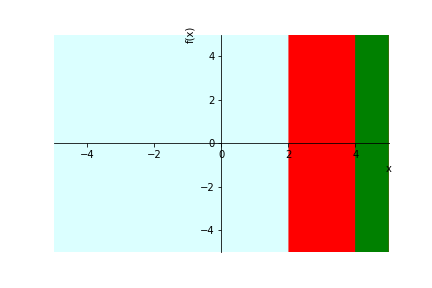
\includegraphics[width=1\columnwidth]{si4}   \end{solution} \part[1]  $ \left\{\begin{matrix}x \geq y \\x + y \geq 4\\x - 2y \leq 8\\\end{matrix}\right. $  \begin{solution}    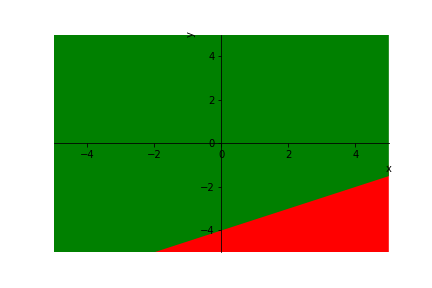
\includegraphics[width=1\columnwidth]{si3}   \end{solution}
        \end{parts}
        \end{multicols}
        \question Averigua el valor de x en los siguientes casos:
        \begin{multicols}{1} 
        \begin{parts} \part[1]  $ \log(2) + \log(11-x^2) = 2\log(5-x) $  \begin{solution}  $ \left [ \frac{1}{3}, \quad 3\right ] $  \end{solution} \part[1]  $ 5\log x - \log 32 = \log(\frac{x}{2}) $  \begin{solution}  $ \left [ 2\right ] $  \end{solution}
        \end{parts}
        \end{multicols}
        \question Resuelve los siguientes sistemas:
        \begin{multicols}{1} 
        \begin{parts} \part[1]  $ \left\{\begin{matrix}3\log x - 2\log y = 10\\\log x + 3\log y = 7\end{matrix}\right. $  \begin{solution}  $ \left [ \left \{ x : 10000, \quad y : 10\right \}\right ] $  \end{solution} \part[1]  $ \left\{\begin{matrix}\log x + \log y = 8 \\\log x - \log y = 2\end{matrix}\right. $  \begin{solution}  $ \left [ \left \{ x : 100000, \quad y : 1000\right \}\right ] $  \end{solution}
        \end{parts}
        \end{multicols}
        
    \end{questions}
    \end{document}
    